\section{L'algoritmo \textit{Nearest Neighbor} (NN)}

Verrà introdotto ora l'algoritmo di \textbf{\textit{Nearest Neighbor} (NN)} per la
classificazione binaria con \textit{feature} numeriche:
$$ \X = \RN^d \qquad\qquad \Y = \{-1,1\} $$

NN non è un'istanza di ERM in quanto non punta a minimizzare $\loss_S$.

\textbf{
L'idea di NN è la sueguente:
\begin{itemize}
    \item Predici ogni punto del \textit{training set} con la propria etichetta;
    \item Predici gli altri punti con l'etichetta del punto del \textit{training set}
        che è più vicino al punto interessato.
\end{itemize}
}

Più formalmente, dato un \textit{training set}:
$$ S = \{(x_1,y_1),\dots,(x_m,y_m)\} $$
l'algoritmo $\Ann$ genera un classificatore $\hnn:\RN \rightarrow \{-1,1\}$ definito
come segue:
$$ \hnn(x) = \text{etichetta $y_t$ del punto $x_t \in S$ più vicino a x} $$

Se a minimizzare la distanza con $x$ sono più punti, si predirrà l'etichetta più
presente tra i putni vicini. Se non c'è una maggioranza di etichette tra i punti
più vicini si predirrà un valore di default $\in \{-1,1\}$.

Presi due punti $x=(x_1,\dots,x_d)$ e $x_t=(x_{t,1},\dots,x_{t,d})$, la distanza
$||x-x_t||$ verrà calcolata tramite la distanza euclidea:
$$||x-x_t|| = \sqrt{\sum_{i=1}^d (x_i-x_{t,i})^2}$$

Ogni classificatore binario $\pred : \RN^d \rightarrow \{-1,1\}$ partiziona $\RN^d$
in due regioni (come mostrato in figura \ref{fig:voronoi}):
$$ \colorbox{orange}{$\{ x \in \RN^d : \pred(x)=1 \}$} \quad , \quad 
   \colorbox{cyan}{$\{ x \in \RN^d : \pred(x)=-1 \}$} $$

\begin{figure}[h]
    \centering
    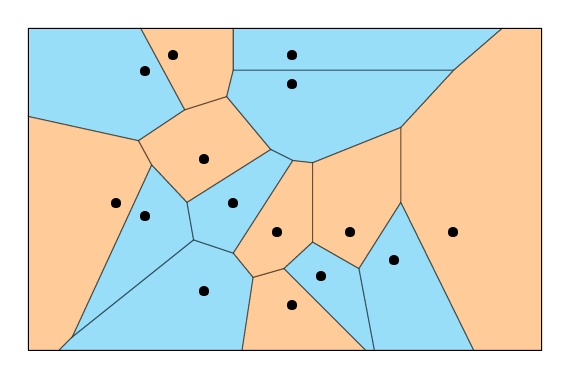
\begin{tikzpicture}[scale=2.8]

    \draw[fill=cyan,opacity=.4](-0.33, 1.33)--(0.18, 1.33)--(0.38, 0.96)--(0.17, 0.82)--(-0.33, 0.93)--(-0.33, 1.33);
    \draw[fill=orange,opacity=.4](-0.33, -0.13)--(-0.33, 0.93)--(0.17, 0.82)--(0.23, 0.71)--(-0.13, -0.07)--(-0.19, -0.13)--(-0.33, -0.13);
    \draw[fill=cyan,opacity=.4](-0.19, -0.13)--(-0.13, -0.07)--(0.42, 0.37)--(0.6, 0.31)--(0.69, 0.2)--(0.64, -0.13)--(-0.19, -0.13);
    \draw[fill=orange,opacity=.4](0.38, 0.96)--(0.57, 1.02)--(0.77, 0.78)--(0.39, 0.54)--(0.23, 0.71)--(0.17, 0.82)--(0.38, 0.96);
    \draw[fill=cyan,opacity=.4](0.23, 0.71)--(0.39, 0.54)--(0.42, 0.37)--(-0.13, -0.07)--(0.23, 0.71);
    \draw[fill=orange,opacity=.4](0.6, 1.33)--(0.6, 1.14)--(0.57, 1.02)--(0.38, 0.96)--(0.18, 1.33)--(0.6, 1.33);
    \draw[fill=cyan,opacity=.4](0.57, 1.02)--(0.6, 1.14)--(1.6, 1.14)--(1.36, 0.88)--(0.96, 0.72)--(0.87, 0.73)--(0.77, 0.78)--(0.57, 1.02);
    \draw[fill=orange,opacity=.4](0.64, -0.13)--(0.69, 0.2)--(0.83, 0.24)--(1.2, -0.13)--(0.64, -0.13);
    \draw[fill=cyan,opacity=.4](0.87, 0.73)--(0.6, 0.31)--(0.42, 0.37)--(0.39, 0.54)--(0.77, 0.78)--(0.87, 0.73);
    \draw[fill=orange,opacity=.4](0.6, 0.31)--(0.87, 0.73)--(0.96, 0.72)--(0.96, 0.36)--(0.83, 0.24)--(0.69, 0.2)--(0.6, 0.31);
    \draw[fill=cyan,opacity=.4](1.2, -0.13)--(0.83, 0.24)--(0.96, 0.36)--(1.17, 0.24)--(1.24, -0.13)--(1.2, -0.13);
    \draw[fill=cyan,opacity=.4](1.82, 1.33)--(1.6, 1.14)--(0.6, 1.14)--(0.6, 1.33)--(1.82, 1.33);
    \draw[fill=orange,opacity=.4](1.36, 0.88)--(1.36, 0.54)--(1.17, 0.24)--(0.96, 0.36)--(0.96, 0.72)--(1.36, 0.88);
    \draw[fill=orange,opacity=.4](2.0, 1.33)--(2.0, -0.13)--(1.69, -0.13)--(1.36, 0.54)--(1.36, 0.88)--(1.6, 1.14)--(1.82, 1.33)--(2.0, 1.33);
    \draw[fill=cyan,opacity=.4](1.24, -0.13)--(1.17, 0.24)--(1.36, 0.54)--(1.69, -0.13)--(1.24, -0.13);
    \draw (-0.33, -0.13)--(2.0, -0.13)--(2.0, 1.33)--(-0.33, 1.33)--(-0.33, -0.13);
    \node at (0.87, 1.2) {\textbullet};
    \node at (0.2, 1.13) {\textbullet};
    \node at (1.13, 0.4) {\textbullet};
    \node at (0.87, 0.07) {\textbullet};
    \node at (0.47, 0.73) {\textbullet};
    \node at (0.2, 0.47) {\textbullet};
    \node at (0.8, 0.4) {\textbullet};
    \node at (0.6, 0.53) {\textbullet};
    \node at (0.87, 1.07) {\textbullet};
    \node at (1.33, 0.27) {\textbullet};
    \node at (0.07, 0.53) {\textbullet};
    \node at (0.33, 1.2) {\textbullet};
    \node at (1.6, 0.4) {\textbullet};
    \node at (0.47, 0.13) {\textbullet};
    \node at (1.0, 0.2) {\textbullet};

\end{tikzpicture}
    \caption{Diagramma di Voronoi in $\RN^2$\label{fig:voronoi}}
\end{figure}